% The PCS.
%%%%%%%%%%

\section{Computation time and the numerical integration of the PCS}

The numerical integration of the PCS using standard quadratic integration for the frame order models is impractical and cannot be used.
A rough estimate for the computation time required for a full analysis of all the frame order models is in the order of 1e$^7$ years.
Therefore a number of tricks have been implemented to speed up the calculations.



% Numerical integration techniques.
%~~~~~~~~~~~~~~~~~~~~~~~~~~~~~~~~~~

\subsection{Numerical integration techniques}

The numerical integration is approximated as
\begin{equation}
    \int f \diff V \approx V \langle f \rangle \pm V \sqrt{\frac{\langle f^2 \rangle - \langle f \rangle^2}{N}} ,
\end{equation}

where the angular brackets are the means.
As the average PCS value in the frame order models is defined as
\begin{equation}
    \overline\delta = \left. \int_S \delta \diff S \right / \int_S \diff S ,
\end{equation}

then
\begin{equation}
    \overline\delta \approx \langle f \rangle \pm \sqrt{\frac{\langle f^2 \rangle - \langle f \rangle^2}{N}} .
\end{equation}

This simply means that the average PCS value of a set of N domain positions which satisfy the constraints of the current model parameter values can be used as the back-calculated PCS value for the model.

The simplest method to calculate the PCS value would be to generate a uniform distribution of domain positions.
The PCS value is calculated for each state in the distribution of N structures and then averaged.
However this technique has non-ideal convergence properties, hence the number N needs to be high to obtain a reasonable estimate of the PCS value.
Two techniques with better convergence properties are the Monte Carlo integration algorithm and the quasi-random integration algorithms.



% Monte Carlo numerical integration.
%~~~~~~~~~~~~~~~~~~~~~~~~~~~~~~~~~~~

\subsubsection{Monte Carlo numerical integration}

As the convergence properties are better than that of a uniform distribution, the Monte Carlo integration algorithm is a viable option for using the PCS in the frame order analysis.
Less states N are required for a reasonable estimate of the back-calculated PCS value.
By randomly selecting N orientations of the domain which lie within the cone half-angle limits, back-calculating the PCS value for each state, and then averaging over all N states, the PCS value for the model can be numerically integrated.
The original implementation used this technique.



% Numerical integration using quasi-random Sobol' points.
%~~~~~~~~~~~~~~~~~~~~~~~~~~~~~~~~~~~~~~~~~~~~~~~~~~~~~~~~

\subsubsection{Quasi-random numerical integration -- Sobol' point sequence}

Although the Monte Carlo numerical integration algorithm is a huge improvement on both the quadratic integration and the uniform distribution numerical integration techniques, it was nevertheless still too slow for optimising the frame order models.
Therefore the quasi-random integration techniques were investigated, specifically using the Sobol' point sequence \citep{Sobol67}.

To implement the numerical integration of the PCS using the quasi-random Sobol' sequence, the LGPL licenced Sobol library of John Burkardt and Corrado Chisari from \url{http://people.sc.fsu.edu/~jburkardt/py_src/sobol/sobol.html} was integrated into the relax library.

For each point coordinate $s_i$, the following functions were used to translate from linear space sampling to rotational space
\begin{subequations}
\begin{align}
    \theta &= \arccos(2s_i - 1), \\
    \phi   &= 2 \pi s_i, \\
    \sigma &= 2 \pi (s_i - \tfrac{1}{2}),
\end{align}
\end{subequations}

where $\theta$ is the frame order tilt angle (the angle of rotation about the x-y plane rotation axis), $\phi$ is the angle defining the x-y plane rotation axis, and $\sigma$ is the torsion angle (the angle of rotation about the z' axis).
Each frame order model uses a different set of $\theta$, $\phi$, and $\sigma$ angles, therefore 1D, 2D, and 3D Sobol' sequences are generated.




% Sobol' oversampling.
%~~~~~~~~~~~~~~~~~~~~~

\subsubsection{Oversampling the Sobol' sequence points}

As generating Sobol' points is computationally expensive, for speed this operation occurs during target function initialisation prior to optimisation.
Hence the Sobol' points are not dynamically generated and a special algorithm is required to ensure adequate 1D, 2D and 3D sampling in the torsion-tilt angle space.
The problem is that as the number of dimensions $M$ increases, the density of a fixed $N$ number of points in the $M$ dimensions decreases.
For example if a fixed value of $N$ is chosen so that the pseudo-ellipse model is properly sampled, then the rotor model will be severely oversampled and take far too long to optimise.
The protocol implemented to avoid this problem is:
\begin{itemize}
    \item Generate $N.Ov.10^M$ points, where $N$ is the maximum number of Sobol' points to be used, $Ov$ is the oversampling factor defaulting to 1, and $M$ is the dimensions of the torsion-tilt angle space.
    \item Convert all Sobol' points into torsion-tilt angles.
    \item Convert all angles to rotation matrices.
\end{itemize}

During optimisation, the following two checks are implemented:
\begin{itemize}
    \item Skip points outside of the limits of the current parameter values.
    \item Terminate the loop over the Sobol' points once N is reached.
\end{itemize}

For most cases, N should be reached.
However if the cone or torsion half-angles are extremely small, then the points used may be less than N.
This is therefore monitored and printed out after each optimisation step.
For these cases, $Ov$ can be increased for better sampling.
This is implemented in the \uf{frame\ufus{}order\ufsep{}sobol\ufus{}setup} user function.




% Parallelization and running on a cluster.
%~~~~~~~~~~~~~~~~~~~~~~~~~~~~~~~~~~~~~~~~~~

\subsection{Parallelization and running on a cluster}

Four different attempts at parallelizing the calculations using the MPI 2 protocol resulted in no speeds up.
In each case, the calculations were up to 2 times slower.
It appears as though the data transfer of the PCS, atomics positions, vectors, etc. between nodes is slower than the calculations.
As parallelization for speeding up the calculations can only achieve around two orders of magnitude faster calculations, the technique was abandoned.




% Frame order model nesting.
%~~~~~~~~~~~~~~~~~~~~~~~~~~~

\subsection{Frame order model nesting}
\index{Frame order!model nesting}

The concept of model nesting is used to hugely speed up the optimisation in the automated protocol.
The most complex models have 15 independent parameters, and performing a grid search over 15 dimensions of the pseudo-ellipse frame order model is not feasible when using PCS numerical integration.
The idea is to use the optimised parameters of a simpler model as the starting point for a more complex model, avoiding the need for a grid search for those copied parameters.
This appears to work as the PCS value is dominated by the average domain position, hence the average domain parameters are very similar in all models.


% Model categories.
\subsubsection{Model categories}

The modelling of the $\sigma$ torsion angle gives a number of categories of related models, those with no torsion, those with restricted torsion, and the free rotors.


\paragraph{No torsion}

When $\sigma = 0$, the following models are defined:
\begin{itemize}
    \item Rigid,
    \item Isotropic cone, torsionless,
    \item Pseudo-ellipse, torsionless.
\end{itemize}


\paragraph{Restricted torsion}

When $0 < \sigma < \pi$, the following models are defined:
\begin{itemize}
    \item Rotor,
    \item Isotropic cone,
    \item Pseudo-ellipse.
\end{itemize}


\paragraph{Free rotors}

When $\sigma = \pi$, i.e.\ there is no torsional restriction, the following models are defined:
\begin{itemize}
    \item Free rotor,
    \item Isotropic cone, free rotor,
    \item Pseudo-ellipse, free rotor.
\end{itemize}


\paragraph{Multiple torsion angles}

This covers a single model -- the double rotor.


% Parameter categories.
\subsubsection{Parameter categories}

There are three major parameter categories -- the average domain position, the eigenframe of the motion, and the amplitude of the motion.


\paragraph{Average domain position}

Let the translational parameters be
\begin{equation}
    \Translateset = \left\{ \aveposx, \aveposy, \aveposz \right\},
\end{equation}

and the rotational or orientational parameters be
\begin{equation}
    \Orientset = \left\{ \aveposa, \aveposb, \aveposg \right\}.
\end{equation}

Two full average position parameter sets used in the frame order models are
\begin{subequations}
\begin{align}
    &\Posset = \Translateset + \Orientset = \left\{ \aveposx, \aveposy, \aveposz, \aveposa, \aveposb, \aveposg \right\}, \\
    &\Possetred = \left\{ \aveposx, \aveposy, \aveposz, \aveposb, \aveposg \right\}.
\end{align}
\end{subequations}


\paragraph{The motional eigenframe}

This consists of either the full eigenframe or a single axis, combined with the pivot point(s) defining the origin of the frame(s) within the PDB space.
The eigenframe parameters themselves are
\begin{subequations}
\begin{align}
    &\Eigensetabc = \left\{ \framea, \frameb, \frameg \right\}, \\
    &\Eigensetax = \left\{ \framet, \framep \right\}, \\
    &\Eigenseta = \left\{ \frameaxa \right\}.
\end{align}
\end{subequations}

The pivot parameter sets are
\begin{subequations}
\begin{align}
    &\Pivotsetone = \left\{ \pivotx, \pivoty, \pivotz \right\}, \\
    &\Pivotsettwo = \left\{ \pivotdisp \right\},
\end{align}
\end{subequations}


\paragraph{The rigid body ordering}

The parameters of order are
\begin{equation}
    \Orderset = \left\{ \conetheta, \conethetax, \conethetay, \conesmax, \conesmaxtwo \right\}.
\end{equation}


% Parameter nesting.
\subsubsection{Frame order parameter nesting in the automated protocol}

\begin{table}
\begin{center}
\caption[Frame order parameter nesting.]{The nesting of frame order model parameters and the resultant grid search dimensionality.  The boxes highlight parameter sets which are optimised in the initial grid search.  The start of each train of arrows are the optimised parameters which will be copied for the more complex model and excluded from the grid search.  The non-nested gird search dimensionality is given in brackets.}
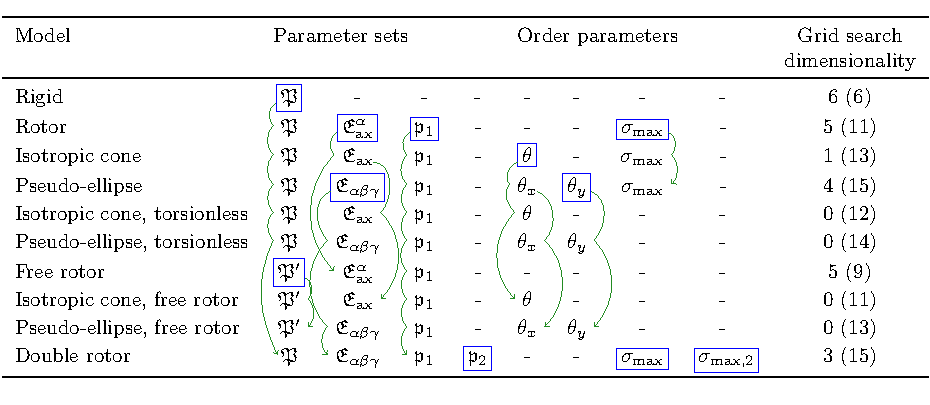
\includegraphics[width=\textwidth]{frame_order/parameter_nesting.ps}
\label{table: frame order parameter nesting}
\end{center}
\end{table}

The parameter nesting used in the automated protocol is shown in table~\ref{table: frame order parameter nesting}.
This massively collapses the dimensionality of the initial grid search.




% PCS subset.
%~~~~~~~~~~~~

\subsection{PCS subset}

Another trick that can be used to speed up the optimisation is to use a subset of all PCS values.
The PCS data for a rigid domain can consist of hundreds of data points.
Rather than using all these values, a very small subset of data points well chosen throughout the 3D structure -- far apart, in rigid locations, and all nearby atoms having a similar value -- can be used for the initial grid search and optimisation.
As the PCS is most sensitive to the average domain position and less to the amplitude of motions, if the subset of atoms is well chosen the optimisation minimum for the subset should be very close to the optimisation minimum for the full data set.
The subset minimum optimisation should be about two orders of magnitude faster as the number of PCS data points are linearly correlated with computation time.
At the end of the analysis, a final stage of slower optimisation using all PCS data can be performed to find the full data set minimum.

In the case of the CaM analyses, a subset of five points was used.
In the peptide bound calmodulin analyses, the H data of residues \{Tyr 99, Val 108, Glu 114, Glu 119, Arg 126\} was used.
As data was not available for the same residues in the free calmodulin analysis, instead the proton data for residues \{Tyr 99, Met 109, Lys 115, Glu 119, Glu 127\} was used.




% Optimisation.
%~~~~~~~~~~~~~~

\subsection{Optimisation}

Due to the numerical integration of the PCS, optimisation is extremely slow.
A number of optimisation techniques can help speed up this part including using a low precision initial grid search, a zooming grid search, an alternating grid search, and zooming precision optimisation.




% Low precision grid search.
%---------------------------


\subsubsection{Low precision grid search}
\index{optimisation!algorithm!grid search!low precision|textbf}

Using 10,000 Sobol' points appears to be the minimum while still delivering about 2-3 decimal places of accuracy for the frame order models (when values are not close to zero).
But rather than using this number of points, 100 can be used in the initial grid search.
This is not accurate enough from the parameter perspective, but is close enough to the real minimum (local or global, see section~\ref{sect: axis permutations} on page~\pageref{sect: axis permutations}).
This speeds up the calculation by two orders of magnitude.



% The zooming grid search.
%-------------------------


\subsubsection{The zooming grid search}
\index{optimisation!algorithm!grid search!zooming|textbf}

This is implemented in relax rather than in the \href{https://gna.org/projects/minfx/}{minfx optimisation library}\index{optimisation!minfx}.
As the grid search is parallelised to run on a cluster using OpenMPI\index{MPI!OpenMPI}, it can sometimes be advantageous to use a fine grid search to find a better optimisation starting position for the Nelder-Mead simplex algorithm\index{optimisation!algorithm!Nelder-Mead simplex}.
Rather than simply increasing the number of increments in the grid search, iteratively performing the grid search while zooming into the optimised parameter values is a more efficient alternative.
This zooming grid search can be seen in the frame order optimisation script on page~\pageref{sect: frame order analysis script}.




% The alternating grid search.
%-----------------------------


\subsubsection{The alternating grid search}
\index{optimisation!algorithm!grid search!alternating|textbf}

For finding the average domain position in the rigid frame order model\index{frame order analysis!rigid model}, an alternating grid search has been implemented in the automated analysis protocol.
The idea is to speed up the slow 6D grid search by first searching over the 3D rotational space, then the 3D translational space.
The grid is then zoomed by one level and alternating grid search is repeated.
As this technique does not guarantee convergence, it is not turned on by default.
The results from the alternation should be carefully checked and the technique avoided if the average domain position is not reasonable.




% Zooming precision optimisation.
%--------------------------------


\subsubsection{Zooming precision optimisation}
\index{optimisation!algorithm!precision!zooming|textbf}

One trick is to perform an iterative optimisation whereby each iteration increases in precision.
For this the function tolerance cutoff for optimisation is used.
But the use of the amount of sampling through the Sobol' sequence can result in much greater speed ups.
The reason is because each point in the Sobol' sequence requires a fixed amount of time to calculate the PCSs for all spins, so time is linearly correlated with the number of points.

Using synthetic CaM data found in \directory{test\_suite/shared\_data/frame\_order/cam/}, the ideal number of Sobol' points was found to be \{100, 1000, 10000\}.
This is combined with a function tolerance cutoff of \{1e$^{-2}$, 1e$^{-3}$, 1e$^{-4}$\}.




% Error analysis.
%~~~~~~~~~~~~~~~~

\subsection{Error analysis}




% Low precision Monte Carlo simulations.
%---------------------------------------


\subsubsection{Low precision Monte Carlo simulations}
\index{Monte Carlo simulations|textbf}

The propagation of errors via Monte Carlo simulation, which is extremely computationally expensive, can also be sped up.
By only using a small number of simulations (50 to 100), 100 Sobol' points, and a function tolerance of 1e-3, the computational time required for Monte Carlo simulations can be dramatically reduced.
However, despite using the lower quality settings, with the current implementation of the frame order theory this error analysis is currently not computationally feasible.
